\providecommand{\qcor}[1]{\ulcorner#1\urcorner}   %
\providecommand{\qcOne}{\mathbf{1}}   %
\providecommand{\qcThree}{\mathbf{3}} %
\providecommand{\cellpair}[5]{$\vcenter{\hbox{\begin{tikzpicture}[x=1.15em,y=1.15em]%
\node (s) at (0,0) {$#1$};%
\node (t) at (4.2,0) {$#2$};%
\draw[->] (0.75,0.32) to[bend left=18] (3.45,0.32);%
\node at (2.1,0.88) {$\scriptstyle#3$};%
\draw[->] (0.75,-0.32) to[bend right=18] (3.45,-0.32);%
\node at (2.1,-0.93) {$\scriptstyle#4$};%
\draw[->] (1.95,0.2) to[bend right=32] (1.95,-0.2);%
\node at (2.85,0) {$\scriptstyle#5$};%
\end{tikzpicture}}}$\ignorespaces}

\section{余笛卡尔纤维化与双纤维化}\label{sec:cocartesian-fibrations-and-bifibrations}

余笛卡尔纤维化与笛卡尔纤维化相对偶，其对偶意义在于：底范畴中的诸箭头以协变方式、
而非反变方式作用于诸\trFiber{}。为了把这一对偶性精确化，回忆第 1 章中的定义
1.2.25：对任意\trInfinityCosmos{} $\mathcal{K}$，存在一个\textbf{\trCodualInfinityCosmos}{}%
$\mathcal{K}^{\mathrm{co}}$，它与 $\mathcal{K}$ 有相同的对象，但其函子空间定义为：
\[
\mathrm{Fun}_{\mathcal{K}^{\mathrm{co}}}(A,B):=\mathrm{Fun}_{\mathcal{K}}(A,B)^{\mathrm{op}}.
\]
$\mathcal{K}^{\mathrm{co}}$ 中的\trIsofibration、\trEquivalence{}与\trTrivialFibration{}%
与 $\mathcal{K}$ 中的相同。$\mathcal{K}^{\mathrm{co}}$ 中的锥形极限与 $\mathcal{K}$ 中的
相同，而 $A\in\mathcal{K}$ 与 $U\in\mathit{sSet}$ 的\trCotensor{}则定义为
$A^{U^{\mathrm{op}}}$。特别地，∞-范畴与 $2$ 的\trCotensor{}定义为
$A^{2^{\mathrm{op}}}$，后者交换了来自箭头∞-范畴与逗号∞-范畴的定义域投影与余定义域
投影。

有了这一结构在手，我们便可简洁地定义：\trInfinityCosmos{} $\mathcal{K}$ 中的余笛卡尔
纤维化，就是一条在\trCodualInfinityCosmos{} $\mathcal{K}^{\mathrm{co}}$ 中定义了%
\trCartesianFibration{}的\trIsofibration{} $p\colon E\twoheadrightarrow B$。于是，5.1--5.3
节中证明的全部结果都发展了\trCocartesianArrow{}、余笛卡尔纤维化以及诸余笛卡尔纤维化之间的
笛卡尔函子的理论。在本节中，我们先纵览其中的若干亮点，然后再把注意力转向%
\emph{\trBifibration}（bifibration），即同时定义\trCartesianFibration{}与余笛卡尔纤维化的
那些\trIsofibration。

\begin{definition}[$p$-余笛卡尔箭头]\label{def:pcocartesian-arrow}
设 $p\colon E\twoheadrightarrow B$ 为一条\trIsofibration。$E$ 中的一支 $X$-形箭头%
$\qcor{\psi}\colon X\to E^{2}$ 是\textbf{$p$-\trCocartesian}，若由\trLeibnizCotensor{}%
的\trPullback{}所定义的虚线映射是一条\trTrivialFibration：
\begin{center}
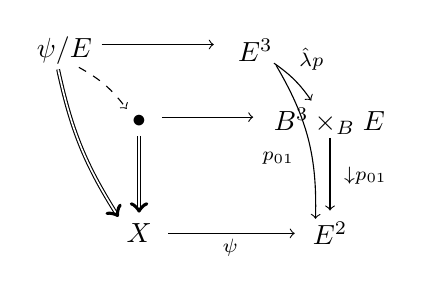
\begin{tikzpicture}[x=1.5em,y=1.5em]
  \node (Ep) at (0,2.7) {$\psi/E$};
  \node (E3) at (4.6,2.7) {$E^{3}$};
  \node (dt) at (1.8,1.0) {$\bullet$};
  \node (BB) at (6.4,1.0) {$B^{3}\times_{B^{\varGamma}}E^{\varGamma}$};
  \node (X)  at (1.8,-1.7) {$X$};
  \node (E2) at (6.4,-1.7) {$E^{2}$};
  \draw[->] (0.9,2.85) -- (3.6,2.85);
  \node at (1.4,2.45) {$\scriptstyle\llcorner$};
  \draw[->,dashed] (0.35,2.3) to[bend left=12] (1.5,1.3);
  \draw[->] (2.35,1.1) -- (4.55,1.1);
  \node at (3.45,1.4) {$\scriptstyle\llcorner$};
  \draw[->] (5.05,2.4) to[bend left=10] (5.95,1.5);
  \node at (5.95,2.5) {$\scriptstyle\hat{\lambda}p$};
  \draw[->] (6.4,0.6) -- (6.4,-1.15);
  \node at (7.25,-0.3) {$\scriptstyle\downarrow p_{01}$};
  \draw[->] (5.1,2.35) to[bend left=16] (6.05,-1.35);
  \node at (5.15,0.1) {$\scriptstyle p_{01}$};
  \draw[double,->] (-0.15,2.25) to[bend right=10] (1.3,-1.3);
  \draw[double,->] (1.8,0.65) -- (1.8,-1.2);
  \draw[->] (2.5,-1.7) -- (5.55,-1.7);
  \node at (4.0,-2.05) {$\scriptstyle\qcor{\psi}$};
\end{tikzpicture}
\end{center}
其中 $\lambda\colon\varGamma\hookrightarrow\qcThree$ 是其像为 $\qcThree$ 中\trSpan{}
$2\leftarrow 0\to 1$ 的那个包含。
\end{definition}

\begin{definition}[余笛卡尔纤维化]\label{def:cocartesian-fibration}
设 $p\colon E\twoheadrightarrow B$ 为一条\trIsofibration。若任何形如下中图的%
\trNaturalTransformation{} $\beta\colon pe\Rightarrow b$ 都容有一个如下右图的
$p$-余笛卡尔提升 $\chi^{\beta}\colon e\Rightarrow\beta_{*}e$，则 $p$ 是一条\textbf{%
余笛卡尔纤维化}：
\begin{center}
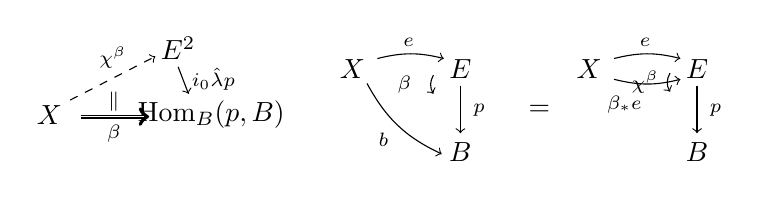
\begin{tikzpicture}[x=1.5em,y=1.5em]
  \node (E2) at (3.1,1.6) {$E^{2}$};
  \node (X)  at (0,0) {$X$};
  \node (HB) at (3.9,0) {$\mathrm{Hom}_{B}(p,B)$};
  \draw[->,dashed] (0.5,0.35) -- node[above,pos=0.5]{$\scriptstyle\qcor{\chi^{\beta}}$} (2.55,1.4);
  \draw[->] (3.1,1.15) -- (3.35,0.5);
  \node at (3.95,0.85) {$\scriptstyle i_{0}\hat{\lambda}p$};
  \draw[double,->] (0.75,-0.05) -- (2.4,-0.05);
  \node at (1.55,0.32) {$\scriptstyle\parallel$};
  \node at (1.55,-0.45) {$\scriptstyle\qcor{\beta}$};
  \node at (6.1,0.7) {$\rightsquigarrow$};
  \begin{scope}[shift={(7.3,0)}]
  \node (E) at (2.6,1.1) {$E$};
  \node (X) at (0,1.1) {$X$};
  \node (B) at (2.6,-0.9) {$B$};
  \draw[->] (0.6,1.35) to[bend left=14] (2.2,1.35);
  \node at (1.35,1.75) {$\scriptstyle e$};
  \draw[->] (2.6,0.7) -- (2.6,-0.45);
  \node at (3.05,0.1) {$\scriptstyle p$};
  \draw[->] (0.35,0.75) to[bend right=18] (2.15,-0.95);
  \node at (0.75,-0.6) {$\scriptstyle b$};
  \draw[->] (1.95,0.95) to[bend right=30] (1.95,0.5);
  \node at (1.25,0.72) {$\scriptstyle\beta$};
  \node at (4.5,0.1) {$=$};
  \end{scope}
  \begin{scope}[shift={(13.0,0)}]
  \node (E) at (2.6,1.1) {$E$};
  \node (X) at (0,1.1) {$X$};
  \node (B) at (2.6,-0.9) {$B$};
  \draw[->] (0.6,1.35) to[bend left=14] (2.2,1.35);
  \node at (1.35,1.75) {$\scriptstyle e$};
  \draw[->] (0.6,0.85) to[bend right=14] (2.2,0.85);
  \node at (0.85,0.25) {$\scriptstyle\beta_{*}e$};
  \draw[->] (2.6,0.7) -- (2.6,-0.45);
  \node at (3.05,0.1) {$\scriptstyle p$};
  \draw[->] (1.95,1.0) to[bend right=30] (1.95,0.55);
  \node at (1.35,0.78) {$\scriptstyle\chi^{\beta}$};
  \end{scope}
\end{tikzpicture}
\end{center}
\end{definition}

同样地，我们只需假设：其定义域穿过 $p$ 的那支\trGenericArrow{}容有一个
$p$-余笛卡尔提升：

\begin{lemma}\label{lem:left-comma-cone-lift}
一条\trIsofibration{} $p\colon E\twoheadrightarrow B$ 是余笛卡尔纤维化，当且仅当
下方左图展示的 $p$ 之上的左逗号锥容有一个如下右图所示的 $p$-余笛卡尔提升 $\chi$：
\begin{center}
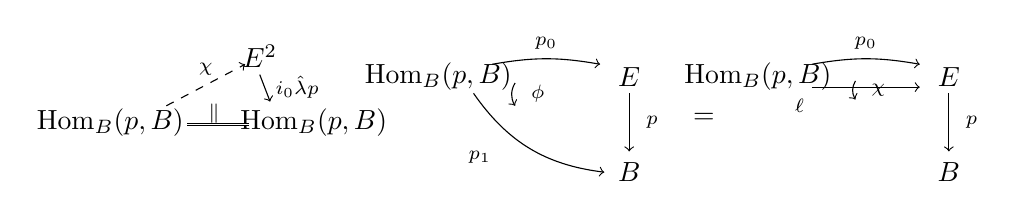
\begin{tikzpicture}[x=1.5em,y=1.5em]
  \node (E2) at (3.6,1.6) {$E^{2}$};
  \node (H1) at (0,0) {$\mathrm{Hom}_{B}(p,B)$};
  \node (H2) at (4.9,0) {$\mathrm{Hom}_{B}(p,B)$};
  \draw[->,dashed] (1.35,0.4) -- node[above,pos=0.5]{$\scriptstyle\qcor{\chi}$} (3.25,1.4);
  \node at (2.5,0.2) {$\scriptstyle\parallel$};
  \draw[->] (3.6,1.15) -- (3.85,0.5);
  \node at (4.5,0.85) {$\scriptstyle i_{0}\hat{\lambda}p$};
  \draw[double] (1.85,-0.05) -- (3.35,-0.05);
  \node at (6.6,0.7) {$\rightsquigarrow$};
  \begin{scope}[shift={(7.9,0)}]
  \node (H) at (0,1.1) {$\mathrm{Hom}_{B}(p,B)$};
  \node (E) at (4.6,1.1) {$E$};
  \node (B) at (4.6,-1.2) {$B$};
  \draw[->] (1.3,1.4) to[bend left=10] node[above]{$\scriptstyle p_{0}$} (3.9,1.4);
  \draw[->] (4.6,0.7) -- (4.6,-0.7);
  \node at (5.15,0) {$\scriptstyle p$};
  \draw[->] (0.85,0.7) to[bend right=24] (4.0,-1.2);
  \node at (1.0,-0.85) {$\scriptstyle p_{1}$};
  \draw[->] (1.85,0.95) to[bend right=30] (1.85,0.4);
  \node at (2.4,0.68) {$\scriptstyle\phi$};
  \node at (6.4,0.1) {$=$};
  \end{scope}
  \begin{scope}[shift={(15.6,0)}]
  \node (H) at (0,1.1) {$\mathrm{Hom}_{B}(p,B)$};
  \node (E) at (4.6,1.1) {$E$};
  \node (B) at (4.6,-1.2) {$B$};
  \draw[->] (1.3,1.4) to[bend left=10] node[above]{$\scriptstyle p_{0}$} (3.9,1.4);
  \draw[->] (1.3,0.85) -- (3.9,0.85);
  \node at (1.0,0.4) {$\scriptstyle\ell$};
  \draw[->] (4.6,0.7) -- (4.6,-0.7);
  \node at (5.15,0) {$\scriptstyle p$};
  \draw[->] (2.35,1.0) to[bend right=30] (2.35,0.55);
  \node at (2.9,0.78) {$\scriptstyle\chi$};
  \end{scope}
\end{tikzpicture}
\end{center}
\end{lemma}

引理 5.4.3 可扩充为余笛卡尔纤维化的一个内部刻画。定理 5.2.8 的对偶要求把诸右伴随
换成：$\Delta_{p}\colon E\to\mathrm{Hom}_{B}(p,B)$ 的一个纤维化左伴随，以及
$i_{0}\hat{\lambda}p\colon E^{2}\to\mathrm{Hom}_{B}(p,B)$ 的一个左伴随右逆（见%
\cref{ex:cocartesian-internal-characterization}）。

命题 5.2.9 与命题 5.2.10 的对偶提供了下面这些例子。

\begin{proposition}[余定义域投影纤维化]\label{prop:projection-fibrations-cocartesian}
对任意\trInfinityCategory{} $A$：
\begin{enumerate}[label=(\roman*)]
\item 余定义域投影函子 $p_{1}\colon A^{2}\twoheadrightarrow A$ 定义了一条余笛卡尔
纤维化。此外，余定义域为 $A^{2}$ 的\trNaturalTransformation{} $\psi$ 是
$p_{1}$-\trCocartesian，当且仅当 $p_{0}\psi$ 可逆。
\item 若 $A$ 容许\trPushout，则定义域投影函子 $p_{0}\colon A^{2}\twoheadrightarrow A$
定义了一条余笛卡尔纤维化，其中诸 $p_{0}$-余笛卡尔胞腔恰是\trPushout{}方块。
\end{enumerate}
\end{proposition}

由此结果与其对偶，当 $A$ 容许\trPushout{}时，定义域投影函子
$p_{0}\colon A^{2}\twoheadrightarrow A$ 既是\trCartesianFibration{}又是余笛卡尔
纤维化。这类映射具有一种特殊性质，我们现在就来探究。

\begin{definition}[\trBifibration]\label{def:bifibration}
一条\trIsofibration{} $p\colon E\twoheadrightarrow B$ 定义了一个\textbf{\trBifibration}，
若 $p$ 既是一条\trCartesianFibration{}又是一条余笛卡尔纤维化。
\end{definition}

投影给出\trBifibration{}的平凡例子。

\begin{example}\label{exa:projection-bifibration}
对任意\trInfinityCategory{} $A$ 与 $B$，投影函子 $\pi\colon A\times B\twoheadrightarrow B$
是一条\trBifibration，其中余定义域为 $A\times B$ 的 2-胞腔是 $\pi$-\trCocartesian{}或
$\pi$-\trCartesian，当且仅当它与投影 $\pi\colon A\times B\to A$ 的复合是一个%
\trIsomorphism。
\end{example}

\begin{proposition}\label{prop:bifibration-fibered-adjunction}
设 $p\colon E\twoheadrightarrow B$ 为一条\trBifibration。则任意\trNaturalTransformation
\cellpair{X}{B}{a}{b}{\beta}
在 $p$ 位于 $a$ 与 $b$ 之上的诸\trFiber{}之间诱导出一个\trFiberedAdjunction：
\begin{center}
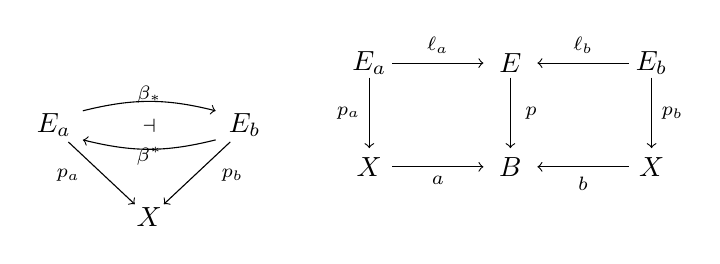
\begin{tikzpicture}[x=1.5em,y=1.5em]
  \node (Ea) at (0,0) {$E_{a}$};
  \node (Eb) at (4.6,0) {$E_{b}$};
  \draw[->] (0.7,0.35) to[bend left=14] (3.9,0.35);
  \node at (2.3,0.75) {$\scriptstyle\beta_{*}$};
  \draw[->] (3.9,-0.35) to[bend left=14] (0.7,-0.35);
  \node at (2.3,-0.75) {$\scriptstyle\beta^{*}$};
  \node at (2.3,0) {$\scriptstyle\dashv$};
  \node (X) at (2.3,-2.2) {$X$};
  \draw[->] (0.35,-0.4) -- (1.95,-1.9);
  \node at (0.35,-1.2) {$\scriptstyle p_{a}$};
  \draw[->] (4.25,-0.4) -- (2.65,-1.9);
  \node at (4.3,-1.2) {$\scriptstyle p_{b}$};
  \begin{scope}[shift={(7.6,0)}]
  \node (Ea) at (0,1.5) {$E_{a}$};
  \node (E)  at (3.4,1.5) {$E$};
  \node (Eb) at (6.8,1.5) {$E_{b}$};
  \draw[->] (0.55,1.5) -- node[above]{$\scriptstyle\ell_{a}$} (2.75,1.5);
  \draw[->] (6.25,1.5) -- node[above]{$\scriptstyle\ell_{b}$} (4.05,1.5);
  \node (X) at (0,-1.0) {$X$};
  \node (B) at (3.4,-1.0) {$B$};
  \node (Xb) at (6.8,-1.0) {$X$};
  \draw[->] (0.55,-1.0) -- node[below]{$\scriptstyle a$} (2.75,-1.0);
  \draw[->] (6.25,-1.0) -- node[below]{$\scriptstyle b$} (4.05,-1.0);
  \draw[->] (0,1.15) -- (0,-0.55);
  \node at (-0.5,0.3) {$\scriptstyle p_{a}$};
  \draw[->] (3.4,1.15) -- (3.4,-0.55);
  \node at (3.9,0.3) {$\scriptstyle p$};
  \draw[->] (6.8,1.15) -- (6.8,-0.55);
  \node at (7.3,0.3) {$\scriptstyle p_{b}$};
  \node at (0.42,0.92) {$\scriptstyle\llcorner$};
  \node at (6.38,0.92) {$\scriptstyle\lrcorner$};
  \end{scope}
\end{tikzpicture}
\end{center}
\end{proposition}

\begin{proof}
记 $\qcor{\beta}\colon X\to B^{2}$ 为由 $\beta$ 诱导的那个函子。注意，定义其在定义域
棱 $a$ 与余定义域棱 $b$ 之上的诸\trFiber{}的那些\trPullback{}可以分解为：
\begin{center}
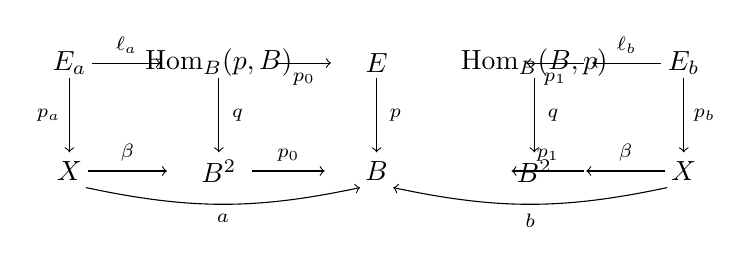
\begin{tikzpicture}[x=1.5em,y=1.5em]
  \node (Ea) at (0,2.6) {$E_{a}$};
  \node (H1) at (3.6,2.6) {$\mathrm{Hom}_{B}(p,B)$};
  \node (E)  at (7.4,2.6) {$E$};
  \node (H2) at (11.2,2.6) {$\mathrm{Hom}_{B}(B,p)$};
  \node (Eb) at (14.8,2.6) {$E_{b}$};
  \draw[->] (0.55,2.6) -- node[above]{$\scriptstyle\ell_{a}$} (2.2,2.6);
  \draw[->] (5.0,2.6) -- node[below]{$\scriptstyle p_{0}$} (6.3,2.6);
  \draw[->] (12.4,2.6) -- node[below]{$\scriptstyle p_{1}$} (11.0,2.6);
  \draw[->] (14.25,2.6) -- node[above]{$\scriptstyle\ell_{b}$} (12.6,2.6);
  \node (X)  at (0,0) {$X$};
  \node (B2a) at (3.6,0) {$B^{2}$};
  \node (B)  at (7.4,0) {$B$};
  \node (B2b) at (11.2,0) {$B^{2}$};
  \node (Xb) at (14.8,0) {$X$};
  \draw[->] (0.45,0) -- node[above]{$\scriptstyle\qcor{\beta}$} (2.35,0);
  \draw[->] (4.4,0) -- node[above]{$\scriptstyle p_{0}$} (6.15,0);
  \draw[->] (12.4,0) -- node[above]{$\scriptstyle p_{1}$} (10.65,0);
  \draw[->] (14.35,0) -- node[above]{$\scriptstyle\qcor{\beta}$} (12.45,0);
  \draw[->] (0,2.25) -- (0,0.45);
  \node at (-0.5,1.35) {$\scriptstyle p_{a}$};
  \draw[->] (3.6,2.25) -- (3.6,0.45);
  \node at (4.05,1.35) {$\scriptstyle q$};
  \draw[->] (7.4,2.25) -- (7.4,0.45);
  \node at (7.85,1.35) {$\scriptstyle p$};
  \draw[->] (11.2,2.25) -- (11.2,0.45);
  \node at (11.65,1.35) {$\scriptstyle q$};
  \draw[->] (14.8,2.25) -- (14.8,0.45);
  \node at (15.3,1.35) {$\scriptstyle p_{b}$};
  \node at (2.55,2.3) {$\scriptstyle\llcorner$};
  \node at (5.0,2.3) {$\scriptstyle\llcorner$};
  \node at (12.15,2.3) {$\scriptstyle\llcorner$};
  \node at (12.65,2.3) {$\scriptstyle\llcorner$};
  \draw[->] (0.4,-0.4) to[bend right=12] node[below]{$\scriptstyle a$} (7.0,-0.4);
  \draw[->] (14.4,-0.4) to[bend left=12] node[below]{$\scriptstyle b$} (7.8,-0.4);
\end{tikzpicture}
\end{center}
定理 5.2.8(ii) 及其对偶给出：函子
$i_{1}\hat{\lambda}p\colon E^{2}\twoheadrightarrow\mathrm{Hom}_{B}(B,p)$ 的一个右伴随
右逆，以及函子
$i_{0}\hat{\lambda}p\colon E^{2}\twoheadrightarrow\mathrm{Hom}_{B}(p,B)$ 的一个左伴随
右逆。把前一\trFiberedAdjunction{}与 $q\colon\mathrm{Hom}_{B}(B,p)\twoheadrightarrow B^{2}$
复合、后一\trFiberedAdjunction{}与 $q\colon\mathrm{Hom}_{B}(p,B)\twoheadrightarrow B^{2}$ 复合，
我们便得到一对可复合的伴随，它们在 $B^{2}$ 之上纤维化：
\begin{center}
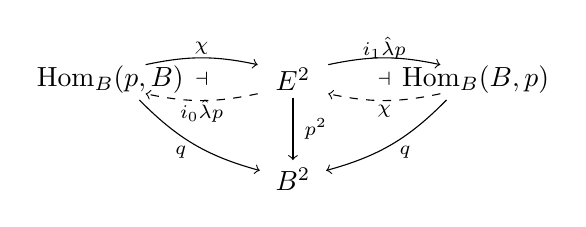
\begin{tikzpicture}[x=1.5em,y=1.5em]
  \node (H1) at (0,0) {$\mathrm{Hom}_{B}(p,B)$};
  \node (E2) at (4.4,0) {$E^{2}$};
  \node (H2) at (8.8,0) {$\mathrm{Hom}_{B}(B,p)$};
  \draw[->] (0.85,0.35) to[bend left=12] (3.55,0.35);
  \node at (2.2,0.75) {$\scriptstyle\qcor{\chi}$};
  \draw[->,dashed] (3.55,-0.35) to[bend left=12] (0.85,-0.35);
  \node at (2.2,-0.78) {$\scriptstyle i_{0}\hat{\lambda}p$};
  \node at (2.2,0) {$\scriptstyle\dashv$};
  \draw[->] (5.25,0.35) to[bend left=12] (7.95,0.35);
  \node at (6.6,0.75) {$\scriptstyle i_{1}\hat{\lambda}p$};
  \draw[->,dashed] (7.95,-0.35) to[bend left=12] (5.25,-0.35);
  \node at (6.6,-0.78) {$\scriptstyle\qcor{\chi}$};
  \node at (6.6,0) {$\scriptstyle\dashv$};
  \node (B2) at (4.4,-2.4) {$B^{2}$};
  \draw[->] (4.4,-0.45) -- (4.4,-1.95);
  \node at (4.95,-1.2) {$\scriptstyle p^{2}$};
  \draw[->] (0.7,-0.5) to[bend right=15] (3.6,-2.2);
  \node at (1.7,-1.75) {$\scriptstyle q$};
  \draw[->] (8.1,-0.5) to[bend left=15] (5.2,-2.2);
  \node at (7.1,-1.75) {$\scriptstyle q$};
\end{tikzpicture}
\end{center}
沿 $\qcor{\beta}\colon X\to B^{2}$ 拉回这一复合伴随，即得所求的\trFiberedAdjunction。
\end{proof}

注意，本证明所给出的伴随函子 $\beta_{*}\dashv\beta^{*}$ 的构造，与注 5.2.7 中所给出的、
2-胞腔 $\beta$ 在 $p$ 的诸\trFiber{}上的作用的描述相吻合。


\subsection*{练习}

\begin{exercise}\label{ex:cocartesian-internal-characterization}
试陈述定理 5.1.7 与定理 5.2.8 的对偶，给出\trCocartesianArrow{}与余笛卡尔纤维化的一个内部
刻画。
\end{exercise}

\begin{exercise}\label{ex:codomain-projection-bifibration}
设 $A$ 是容许\trPullback{}的\trInfinityCategory。由命题 5.2.10 与%
\cref{prop:projection-fibrations-cocartesian}，余定义域投影函子
$p_{1}\colon A^{2}\twoheadrightarrow A$ 是一条\trBifibration。试描述由 $\mathrm{h}A$ 中的
一支箭头 $\alpha\colon x\to y$ 所诱导的伴随里\trLeftAdjoint{}与\trRightAdjoint{}的
作用：
\begin{center}
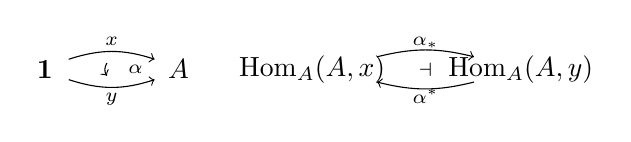
\begin{tikzpicture}[x=1.15em,y=1.15em]
  \node (o) at (0,0) {$\qcOne$};
  \node (A) at (4.2,0) {$A$};
  \draw[->] (0.75,0.32) to[bend left=18] (3.45,0.32);
  \node at (2.1,0.88) {$\scriptstyle x$};
  \draw[->] (0.75,-0.32) to[bend right=18] (3.45,-0.32);
  \node at (2.1,-0.93) {$\scriptstyle y$};
  \draw[->] (1.95,0.2) to[bend right=32] (1.95,-0.2);
  \node at (2.85,0) {$\scriptstyle\alpha$};
  \node at (6.4,0) {$\rightsquigarrow$};
  \begin{scope}[shift={(8.4,0)},x=1.3em,y=1.3em]
  \node (Hx) at (0,0) {$\mathrm{Hom}_{A}(A,x)$};
  \node (Hy) at (5.8,0) {$\mathrm{Hom}_{A}(A,y)$};
  \draw[->] (1.8,0.35) to[bend left=14] (4.5,0.35);
  \node at (3.15,0.75) {$\scriptstyle\alpha_{*}$};
  \draw[->] (4.5,-0.35) to[bend left=14] (1.8,-0.35);
  \node at (3.15,-0.75) {$\scriptstyle\alpha^{*}$};
  \node at (3.15,0) {$\scriptstyle\dashv$};
  \end{scope}
\end{tikzpicture}
\end{center}
\end{exercise}

